\documentclass[rnd]{mas_proposal}
% \documentclass[thesis]{mas_proposal}

\usepackage[utf8]{inputenc}
\usepackage{amsmath}
\usepackage{amsfonts}
\usepackage{amssymb}
\usepackage{graphicx}
\usepackage{placeins}

\title{Advancing 2D LiDAR-based Indoor Localization using Surface Normal-constrained Particle Filters}
\author{Waseem Mohammed}
\supervisors{Prof. Dr Paul G. Plöger\\M.Sc. Deebul Sivarajan Nair}
\date{August 2023}

% \thirdpartylogo{path/to/your/image}

\begin{document}

\maketitle

\pagestyle{plain}

\section{Introduction}
Particle filters represent a vital tool in the domain of localization, offering a robust approach to estimating the position and orientation of robot within various environments. In particle filters, the belief of the robot’s pose is represented by a set of weighted samples that are updated recursively through Bayesian filtering. This allows for the representation of arbitrary multimodal uncertainty distributions that may arise when operating in challenging environments, unlike with Kalman filters which are restricted to unimodal Gaussians\cite{772544}. However, Particle filters encounter distinct challenges that can effect their performance. One significant obstacle is the widely recognized issue of particle degeneracy, where the available particles become insufficient to accurately represent the true state of the system. This phenomenon poses a threat to localization accuracy, potentially yielding suboptimal results.

Another key challenge is the inherent trade-off between accuracy and robustness observed within conventional particle filters. This dilemma becomes pronounced when addressing map discrepancies, introducing a delicate balance that impacts localization outcomes.  

While addressing map discrepancies for improved robustness is conceivable through modifications to the observation model, it is imperative to acknowledge that such adjustments can inadvertently diminish the informativeness of the model, potentially resulting in a corresponding decline in accuracy\cite{Markov_Localization} \cite{7759301}.

Addressing these challenges necessitates innovative solutions. One notable approach involves the efficient implementation of an optimal particle filter. This optimization leverages surface normals harnessed from 3D LiDAR data, enhancing the filter's performance. By integrating surface normal information into the particle filter process, this approach bridges the gap between accuracy and robustness, providing a more reliable solution for indoor localization \cite{10160274}.

This research and development project aims to extend the existing localization framework by drawing inspiration from the successful integration of surface normals in 3D systems. This integration has demonstrated great promise in achieving accurate indoor localization. Building upon this success, the project aims to transfer and apply these principles to a 2D framework. By doing so, the project endeavors to enhance the precision and reliability of indoor localization, particularly in scenarios where the use of 3D LiDAR setups might be impractical or cost-prohibitive. Through the incorporation of surface normal information into the particle filter process, this project aspires to address the challenges posed by conventional particle filters, ultimately leading to an enriched and more effective localization methodology.

The core objectives of this project encompass both the theoretical and practical aspects of integrating surface normal constraints into 2D LiDAR-based particle filters. The research will delve into designing novel methodologies that capture the essence of surface normals in a 2D context, while also addressing challenges unique to this scenario. Subsequently, the proposed methodologies will be rigorously benchmarked and tested, assessing their impact on the accuracy and performance of the localization system. This comparative analysis will provide empirical evidence of the benefits derived from surface normal incorporation in the 2D LiDAR setting, ultimately highlighting its potential to enhance the precision and dependability of indoor localization.

\section{Related Work}

The field of optimal localization and particle filtering has witnessed substantial progress in tackling complex challenges inherent to robotics, such as particle degeneracy, map discrepancies, and computational efficiency. Noteworthy advancements have been made by researchers, offering diverse strategies to address these issues.

Grisseti et al.\cite{4084563} introduced an intriguing approach that centers around approximating the optimal proposal distribution using scan matching techniques. This technique leverages sample-based methods to approximate the proposal distribution, a crucial step to minimize particle degeneracy – a common phenomenon where the available particles become insufficient to accurately represent the true state of the system. While effective, this technique introduces additional computational complexity due to the need for multiple sampling steps and the evaluation of observation likelihoods for each particle.

Blanco et al.\cite{article}, recognizing the computational challenges posed by the scan matching approach, presented an innovative alternative. This approach refrains from relying on scan matching or Gaussian approximations, thereby offering an avenue to mitigate computational overhead. However, similar to the previous method, this technique faces challenges in maintaining efficiency, particularly when handling non-parametric observation models that require point-wise evaluation of likelihoods.

The handling of dynamic obstacles during localization, a significant aspect of map discrepancies, was effectively addressed by Jianchao et al.\cite{8028452}. Their approach involves the integration of a motion detection module, allowing the system to disregard scan points stemming from dynamic objects. Nonetheless, this method is most effective for unmapped objects in motion during localization, leaving a gap in scenarios involving semi-static objects or uncertainties in the robot's pose.

Temporary maps, as explored by other researchers \cite{5648920} \cite{6907433}, introduce a promising solution for handling observations of semi-static objects. These maps serve as a buffer, enabling the system to better incorporate and utilize such observations. However, the viability of these approaches rests on accurate particle filter estimates, potentially limiting their robustness in scenarios characterized by pose uncertainty.

A more comprehensive perspective was adopted by Tipaldi et al.\cite{Tipaldi2013LifelongLI}, who embraced environment estimation within multi-session SLAM. This extension involved encompassing the environment as part of the state variable. While this approach showed promise in theory, the increased complexity of the map introduced heightened computational demands, potentially challenging its real-world applicability.

In the context of the present study, we extend the proven principles of optimal 3D localization into the domain of 2D environments. Our novel approach harnesses the power of a closed-form Gaussian approximation of the optimal proposal distribution. This is obtained by utilizing surface normal information in LiDAR scans and maps to derive an efficient Gaussian
approximation of the observation model \cite{10160274}. This innovation lends itself well to efficient 2D implementation, a crucial aspect when considering computational resource constraints.

Moreover, we draw inspiration from the integration of surface normal information extracted from LiDAR scans and maps. This information allows us to derive a precise Gaussian approximation for the observation model, contributing to addressing the challenges of map discrepancies and particle degeneracy.

To comprehensively address map discrepancies, we introduce an innovative strategy involving two distinct observation models. These models are strategically employed within both the particle propagation and weight update stages of the particle filter. This dual-model integration significantly bolsters the localization process, enhancing accuracy and robustness while incurring only a minimal increase in computational overhead\cite{10160274}.

In summary, our work not only builds upon the advancements in optimal 3D localization and map handling techniques but also offers a refined adaptation of these principles for 2D scenarios. By incorporating a closed-form Gaussian approximation and an inventive dual-model observation integration, our approach presents a promising avenue to substantially enhance the accuracy, reliability, and efficiency of 2D LiDAR-based indoor localization.

\section{Problem Statement}
Particle filters have emerged as a crucial technique for accurate robot localization in various environments, offering the ability to represent multimodal uncertainty distributions. However, the efficacy of particle filters in addressing challenges specific to 2D LiDAR-based indoor localization remains an open question. Notably, the widely observed issues of particle degeneracy and the inherent accuracy-robustness trade-off when handling map discrepancies pose substantial hurdles to achieving precise and reliable 2D localization results.
In the context of 2D LiDAR-based indoor localization, the most prevalent particle filtering algorithm is the Sampling Importance Resampling (SIR) filter\cite{Rubin1988UsingTS}. This algorithm entails three main steps:

\textbf{Sampling}: For each particle $i$ with pose $x^i_t$ and weight $w^t_i$ at time step $t$, a new sample pose is drawn from a proposal distribution:
\begin{equation}
    x^{i}_{t} \sim {q}(x_{t} \mid x^{i}_{t-1},z_{t},u_{t})
\end{equation}
where $u_t$ and $z_t$ are the control input and observations at time $t$, respectively.

\textbf{Weight Update}: The particle weights are updated according to:

\begin{equation}
    w_t^i \propto w_{t-i}^{i}\frac{p(z_t \mid x^i_t)p(x^i_t \mid x^i_{t-1},u_t)}{q(x^i_t \mid x^i_{t-1},z_t,u_t)}
\end{equation}
where $p(x^i_t \mid x^i_{t-i},u_t)$ corresponds to the robot’s motion model and $p(z_t \mid x^i_t)$ corresponds to the observation model.

\textbf{Resampling}: A new set of particles is drawn from the existing particle set with probabilities proportional to the weights in a resampling step, addressing particle degeneracy.
The challenges arise from both the particle degeneracy problem and the accuracy-robustness trade-off when addressing map discrepancies.

\subsection{Particle Degeneracy Problem}
In 2D localization, particle degeneracy stems from the utilization of the robot's motion model $p(x^i_t \mid x^i_{t-1},u_t)$ as the proposal distribution. This approach simplifies weight updates based on observation likelihoods but leads to an inefficient allocation of particles within the high-likelihood regions of the observation model. This inefficiency becomes more pronounced when sensor measurements provide informative data. For instance, the standard particle filter might assign negligible weights to particles drawn from the motion model, limiting accurate pose estimation.
Moreover, particle degeneracy impacts the robustness of the system. Consider a scenario where the robot navigates through a corridor with ambiguous LiDAR measurements. The particle set should ideally represent the uncertainty in odometry along the corridor, but the noisy motion model-based proposal distribution introduces errors perpendicular to the corridor. As particles with higher errors in the perpendicular direction are assigned lower weights, resampling might lead to the depletion of particles around the actual robot pose, compromising recovery during unambiguous measurements.

\subsection{Map Discrepancies}
Handling map discrepancies presents another challenge. In 2D systems, environmental changes can violate the Markov assumption used in calculating observation likelihoods, causing localization failures. Addressing such discrepancies often involves adjusting the observation likelihood calculations based on the likelihood of observing scan points from unmapped obstacles. While this approach enhances robustness, it can compromise accuracy by disregarding informative scan points.

\subsection{Aims and Objectives}
The overarching goal of this research and development project is to extend the successful principles of optimal 3D localization to the domain of 2D LiDAR-based indoor localization by devising innovative solutions that address the particle degeneracy problem and the accuracy-robustness trade-off inherent in handling map discrepancies. Building upon the advancements achieved in 3D optimal localization, this project aims to implement and adapt the same principles to the 2D framework.
To achieve this, the project aims to:
\begin{itemize}
    \item Develop an efficient optimal particle filter-based localization system tailored to 2D LiDAR data.
    \item Integrate surface normal constraints into the optimal particle filter framework to enhance accuracy and robustness.
    \item Design and implement a high-fidelity observation model for accurate particle propagation.
    \item Devise a low-fidelity observation model to ensure robust weight updates while handling map discrepancies.
    \item Evaluate the proposed system's performance against a standard particle filter-based baseline in challenging localization scenarios, utilizing both simulation and real-world data.
\end{itemize}

By achieving these objectives, the project aspires to establish a novel 2D localization approach that significantly enhances accuracy, robustness, and efficiency in indoor environments. Through the integration of surface normal information and the refinement of observation models, the project seeks to propel 2D LiDAR-based indoor localization to new heights of precision and dependability.

\section{Project Plan}

\subsection{Work Packages}
The bare minimum will include the following packages:
\begin{enumerate}
    \item[WP1] Literature Study
    \item[WP2] Understanding Localization with Standard Particle Filters and Monte Carlo Localization
    \item[WP3] Understanding Localization with Optimal Particle Filters Using Surface Normals in 3D
    \item[WP4] Implementation of Existing 3D Optimal Particle Filter
    \item[WP5] Simulation Environment Setup
    \item[WP6] Algorithm Implementation for 2D LiDAR
    \item[WP7] Surface Normal Extraction for 2D LiDAR Data
    \item[WP8] Robustness Testing and Scenario Variations
    \item[WP9] Evaluation of approach and comparison with similar approaches
    \item[WP10] Project Report
\end{enumerate}

\subsection{Milestones}

\begin{enumerate}
    \item[M1] Literature review completed and best practice identified
    \item[M2] Conceptual Understanding Achievement
    \item[M3] 3D Optimal Particle Filter Implementation and Framework Preparation
    \item[M4] Adapting 3D Implementation for 2D Lidar and Integrating 2D Surface Normals
    \item[M5] Benchmarking, Testing, and Real-world Validation
    \item[M6] Report submission
\end{enumerate}
\newpage
\subsection{Project Schedule}
\FloatBarrier
\begin{figure}[h!]
    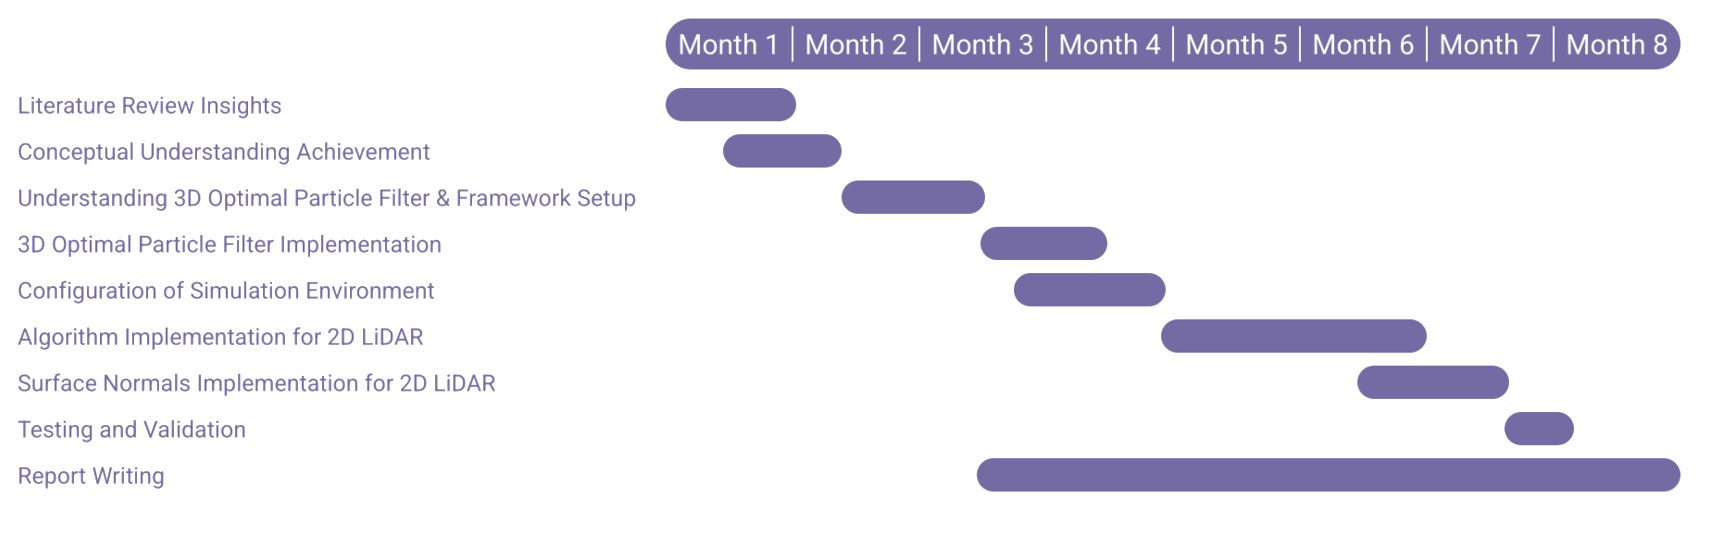
\includegraphics[width=\textwidth]{images/Timeline.png}
    \caption{Project Schedule}
    \label{fig:myfigure}
\end{figure}
\FloatBarrier
\subsection{Deliverables}

\subsubsection*{Minimum Viable}
\begin{itemize}
    \item Literature Review Insights
    \item Conceptual Understanding Achievement 
    \item Implementation and Framework Setup of 3D Optimal Particle Filter
    \item Configuration of Simulation Environment
    \item R\&D Report Documentation
\end{itemize}

\subsubsection*{Expected}
\begin{itemize}
    \item Algorithm Implementation for 2D LiDAR
    \item Implementation of Algorithm for 2D LiDAR
    \item Extraction of Surface Normals from 2D LiDAR Data
    \item Testing for Robustness and Varied Scenarios
\end{itemize}

\subsubsection*{Desired}
\begin{itemize}
    \item Benchmarking
    \item Testing, and Real-world Validation 
    \item Using different approaches for map
\end{itemize}

\newpage
\nocite{*}

\bibliographystyle{plainnat} % Use the plainnat bibliography style
\bibliography{bibliography.bib} % Use the bibliography.bib file as the source of references

\end{document}
